%This section discusses our preliminary results.
%This file should be included in doc using \input{file}
\section{Preliminary Results}
\subsection{SimuLink System Models}
Using SimuLink, a model of the quadcopter system and control system was built.  This was used to perform preliminary hovering tests.  The SimuLink model was broken down into several blocks.  Each of these blocks was built to handle key aspects of the system.  The system can be seen in it's current state in the following figure.  Each of the blocks shown are discussed in detail below.

\begin{figure}[h]
  \centering
  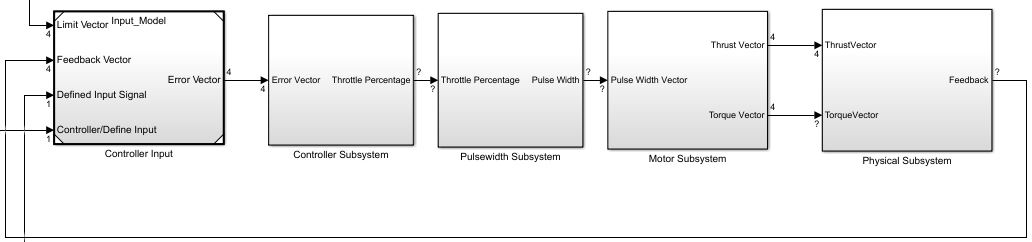
\includegraphics[scale=0.45]{system_arch.jpg}
  \caption{SimuLink Control System Architecture}
  \label{fig:sys_arch}
\end{figure}

%\begin{itemize}
%  \item{Input_Model.slx}
%  \item{Controller_Model.slx}
%  \item{Motor_Characterization.slx}
%  \item{Multibody_Base.slx}
% \end{itemize}
\subsubsection{Input Model}
This block is the front end of the simulation.  The four inputs to this block specify the origin of the control signal as well as the limits or sensitivity on the signal.  As well as a port for sensor feedback.  The final output is the error vector for the control system.  The inputs are discussed in further detail below:
\begin{enumerate}
	\item \textbf{Limit Vector}:  This input takes a four dimensional vector of limits.  These limits respectively apply to roll, pitch, yaw, and altitude.  Roll, pitch, and yaw should be specified in degrees.
	\item \textbf{Feedback Vector}: This input takes a four dimensional vector of the current values of roll, pitch, yaw, and altitude.  This is then subtracted from the control signal to create the error signal.
	\item \textbf{Defined Input Signal}:  This input takes a four dimensional vector of control signal.  Values for this should be normalized between -1 and 1.
	\item \textbf{Controller/Define Input}:  This input specifies whether to use a control signal from \textbf{Input 3} or from a controller (e.g. Joystick, DualShock gamepad) attached to the computer.
\end{enumerate}

\subsubsection{Controller Model}
This subsystem contains the control system for the quadcopter.  It currently consists of a PI controller for all four of our control signals.  The gain values for these controllers have not yet been finely tuned.  The outputs of the controllers are limited to be between 0 and 100.  This is to represent a percentage of our throttle.

\subsubsection{Pulse Width Subsystem}
This subsystem takes the percentage of throttle and translates it into a pulse width within the applicable range for our speed controller.  Our lowest throttle is at 1127 $\mu s$ while our highest throttle is at 1860 $\mu s$.  Our output is given by the equation:

\begin{align*}
	PulseWidth &= Throttle\% \cdot (1860 \mu s - 1127 \mu s) + 1127 \mu s 
\end{align*}

\subsubsection{Motor Characterization}
This subsystem determines the thrust and torque from each motor depending on their respective pulse width.  Thrust is determined by using a lookup table; extrapolated from our experimental data.  As we were unable to characterize the torque or the speed of the rotor, the output torque is an estimate based on the value of the thrust.

\subsubsection{Physical Subsystem}
This subsystem houses the physical simulation that has been created using SimuLink's Simscape Multibody package.  It currently consists of a rudimentary visualization of a quadcopter.  No more complex than a cross representing the body between the motors.  In the simulation a force and torque is applied at the end of these arms to simulate the action created by the motors.  
The inputs for this subsystem are a vector of the magnitude of the motor thrusts and a vector of magnitude of the motor torques.  The simulation accounts for the direction of rotation of the motors by applying the torques along either the X or Y axis of the model, depending on the rotation.  The subsystem also outputs the current roll, pitch, yaw, and altitude to be fed back.

\subsection{Hover Test}
Using the models and systems discussed in the previous subsection, our preliminary flight simulation was constructed.  The SimuLink model Dynamic\_Simulation.slx was created.  The altitude controller was tested by providing a step input.  After some tuning of the controller, we were able to obtain the following step response.

\begin{figure}[h]
	\centering
	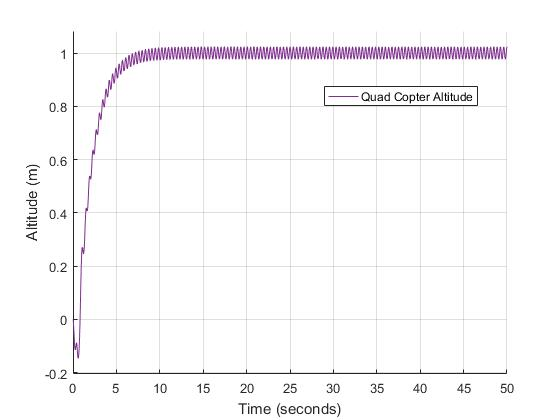
\includegraphics[scale = 0.5]{stepresponse.jpg}
	\caption{Hovering Step Response, for 1 metre altitude.}
	\label{fig:1m_step}
\end{figure}

Currently the simulation does not account for a hard stop at 0 altitude.  At the beginning of the response above, the quadcopter can be seen to fall briefly.  Once the rotors have generated sufficient thrust, the quadcopter continues towards the requested 1 meter altitude.

  \subsection{Proof of Concept and Testing Performed}
  
  To date, several tests and proof of concepts have been performed to determine methods of controlling hardware, limitations of the hardware or software and to determine feasibility of communication protocols. The test subjects include:
  
\begin{itemize}
  \item{PWM}
  \item{Electronic Speed Controller}
  \item{Motor Lift Characteristics}
  \item{Wi-Fi Range}
  \item{I2C Communication Channel}
  \item{Playstation Controller Integration}
 \end{itemize}
  
  \subsubsection{PWM}
  
Using an Arduino micro controller, a potentiometer and a simple DC motor, a circuit was devised to test a PWM output of the Arduino to drive a motor circuit. The motor circuit was isolated using a mosfet as the switching operator and a diode to ensure there would be no damaging back emf in the system. A 9V battery powered the isolated circuit.
  
Through programming, the voltage across the potentiometer was taken into the Arduino as an analog input and mapped to a digital output as a PWM duty cycle. The script was successful in providing an input controlled PWM value to the motor. The code was modified to suit the needs of the electronic speed controllers by applying an input controlled pulse width as a function of time in replacement of a duty cycle as the ESC's require a pulse width range of 1060 $\mu$s and 1860 $\mu$s.

  
  \subsubsection{Electronic Speed Controller}
  
The Afro ESC 12Amp BEC UltraLite Multirotor ESC V3 was tested at St. Mary's University with the assistance of Dr. Rhinelander. An Arduino running a script to map a potentiometer to a PWM duty cycle was used as an attempt to control the motor through the ESC. A 12V power supply fed the ESC while the Arduino controlled the duty cycle of the speed controller producing a voltage output to control the motor speed. 

The ESC testing was successful, the testing proved the Arduino's capability to control the motor with a variable input. The testing had flaws as a PWM duty cycle was used instead of a timed pulse width input. The duty cycle had potential of operating correctly as the range of times could have been calibrated to a range in the duty cycle although this method proved to be difficult due to low values causing the ESC to enter calibration mode. The script used to operate the ESC was re-written as a timed pulse width to ensure complete compatibility and ease of future integration.The pulse width script was tested using the ESC and was successful. The provided motor was successfully driven under no load conditions for the full range of pulse width values.

 \subsubsection{Motor Lift Characteristics}
 
 Using a 12V power supply, the provided ESC and the Multi-Star Elite motor the characteristics of the motor's lifting capacity were tested. A weight was attached to a support system with the motor and blade seated on top. The apparatus was placed on a scale and the scale's reading was zeroed. As the rotor speed increased, the reduction in weight read by the scale was considered the lift capacity.
 
 The test was performed beginning at a pulse width of 1127$\mu$s which was found through experimentation to be the cut in pulse width for motor operation. The test was performed at increments of 25$\mu$s. The resultant current draw values and lift values were documented. The lift values were used to create a simulink lookup table to characterize the motor's available force for simulation purposes. 
 
 During the load testing, it was noticed that the current draw from the individual motor was high. The power supply being used had a current limit of 3 A therefore the maximum current draw allowed during testing was 2.95 A to ensure no brown out due to lack of supply. The current limiting factor resulted in the test ending at a pulse width of 1525$\mu$s and a lift value of 137.5g.

  \subsubsection{Wi-Fi and Bluetooth Range}
  
  A simple proof of concept regarding the range of Wi-Fi communications was performed. The test incorporated a a Wi-Fi communicating camera tethered to a Wi-Fi output from a cell phone. A user walked down Spring Garden holding the cell phone and found the approximate distance at which the phone and the camera lost communication. It was found that the range was approximately 100 ft with line of sight available but no Wi-Fi boosting technology. Bluetooth communications were also tested using the Raspberry Pi 3 connected to a Playstation 4 controller although the communication channel held a strong connection for only approximately 10 ft, this distance was considered insufficient for the scope of the project.
  
  
  \subsubsection{I2C Communication Channel}
  
  The flight controller will consist of both an Arduino micro controller and a Raspberry Pi 3 Linux based computer system. The flight controller will require a communication channel between each component to transmit data between each system. To enable these communications, an I2C bus is planned to be utilized.
  
  The I2C bus was enabled on the Raspberry Pi and a sample open source script was run on the Arduino to begin I2C communications. The test resulted in the Raspberry Pi recognizing the Arduino on I2C bus.
  
  
  \subsubsection{Playstation Controller Integration}
  
  Using an open source python script, a Playstation 4 controller was integrated with the built in Bluetooth communication channel of the Raspberry Pi 3. All inputs available from the Playstation controller were taken in as values to the Raspberry Pi, confirming the compatibility of systems. Based on the Playstation controller integration testing, the feasibility of the Bluetooth communication was put into question. Although successful, it was decided that based on range constraints, Bluetooth would not be used as the communication channel, a hardwired serial connection to a base station will be utilized. 
